\documentclass[a4paper]{article}

\usepackage[utf8]{inputenc}

\usepackage{url}
\usepackage[]{hyperref}

\usepackage{caption}

\usepackage{listings}

\usepackage{color}

% *** GRAPHICS RELATED PACKAGES ***
%\usepackage[pdftex]{graphicx}
\usepackage{graphicx}
%\usepackage[dvips]{graphicx}
% to place figures on a fixed position
\usepackage{float}

\usepackage[margin=1in]{geometry}

\title{Cloud systems – syllabus}
\author{}
\date{}


\begin{document}

\maketitle

\tableofcontents

\section{Cloud Systems}

The spread of the cloud-based computing is unquestionable in recent years, its penetration has caused the growth of the
number and size of datacenters. Facebook, Google, Microsoft, Apple, Oracle, Amazon, etc. run data centers made out of
tens of thousands of computers, and offer a wide variety of services from back-end support of mobile applications
through Virtual Machines (VMs) to content-distributing systems. Needless to say, those smaller data centers are spreading
too, which make the IT infrastructure of even a smaller firm much more simple and manageable by creating a private
cloud. Beside the great cloud-providers (Amazon, Google, Microsoft, etc.) there are many open-source projects, which
are capable of creating, managing and installing cloud-based systems. One of these is the widespread and constantly
developed system called OpenStack. As a combination of public and private cloud, there is a third system called hybrid
cloud, which revolves around the idea that the very sensitive data (e.g. email, data of employees) stay within the
firm, while the less critical items get transported into a public cloud.

Considering the type of the cloud service, the following categories were defined: a cloud-provider can provide Software
as a Service (SaaS), Platform as a Service (PaaS) and Infrastructure as a Service (IaaS), beside the many other
solutions that are less wide spread. The easiest to imagine is the infrastructure service, because in this situation
the customer rents VMs, which they can utilize. The price of the rent is determined by the engaged
resources. OpenStack uses the IaaS solution too, that is it assures a virtual infrastructure for its users: the users
are able to exploit the computing capacity of the VMs (on which they are able to install any optional
software), to manage the storage and virtual networks.

The Platform as a Service is a bit more complicated, this is usually chosen by the renters to handle an own
application, because they don't want to deal with installing and configuring the operating system and handling and
updating the main components of the system, but with running their own application. The point of the software-based
service is that the customer uses a software, an application that is running in the cloud. A good example for this is
Google Docs, but so is any email service.

The main point of the cloud is that the services aren't run on a dedicated hardware, but are distributed among multiple
physical computers, which are parts of one system.  From the angle of the user of the cloud, this infrastructure is
hidden, they only see an integrated interface, as if the service was run in a conventional environment, on one or
multiple computer(s). Through this interface, the user is able to manage their administrative tasks related to the
cloud, and those that are required to run such a cloud, while the provider (the operator of the cloud) isn't needed to
interfere anyhow, this is (for a clear reason) an interest of the provider too. In addition, the user of the cloud
benefits in other ways, such as high availability, load-distribution, redundancy, scalable services.

Scalability means that in case of growth in the traffic of the customer, the capacity of the service installed into the
cloud is increasable too. This means that just because of a period with expectedly high traffic, getting expensive
hardware with high capacity - which would be unnecessary after this period - isn't required. These capacities can be
adjusted, there is always an option to start or stop a VM, to modulate the available capacity. This is
mostly relevant in those services, which do not have a consistent load.

Virtualization is an important element of the cloud systems. With virtualization, we are able to run isolated
environments simultaneously and independently on a physical computer, which is seen as a separate operating system from
the angle of the application. Using this method, we can exploit formerly unexploited server capacity, because usually
less physical servers are also enough to carry out the same amount of job, and this way the computers use less energy.

\section{OpenStack}

OpenStack is an open-source, free software-package for creating private and public IaaS clouds. Many famous firms,
universities and research-centers use OpenStack (e.g. HP, PayPal, CERN, Harvard University, Wigner Datacenter).
OpenStack is constantly evolving, there is a new version with significant corrections released twice a year. It usually
handles a large amount of computing and storage capacity and network devices, while creating a datacenter over the
physical infrastructure. The infrastructure-granting components in OpenStack consist of three main types: compute,
networking and storage (Figure~\ref{fig:oscomponents}). Dashboard grants the on-line administrative interface for
users, this can be used to configure resources and create services. The tasks of the servers granting computing
capacity are running VMs and services, as well as receiving commands coming from the administrative
interface. The component handling the network is responsible for setting up the network between VMs, as
the storage component helps us to assign separate storages to our VMs (in a minimal configuration this is
optional).

\begin{figure}[H]
    \centering
    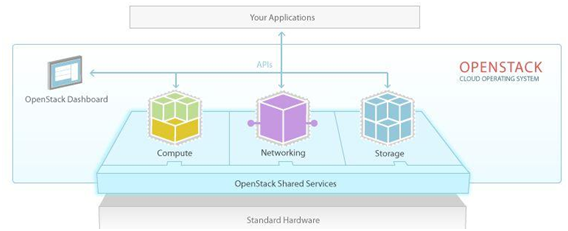
\includegraphics[width=0.9\textwidth]{figures/components.png}
    \caption{OpenStack basic components}
    \label{fig:oscomponents}
\end{figure}

The Dashboard is the on-line user interface, which provides the opportunity for the users to create and manage virtual
computers, thus accessing the resources of the system. A different method for accessing the system is using the
command-line or programming interface of OpenStack. The network configuration and connections (how the virtual
computers should connect to each other or to internal/external networks) can also be adjusted through the on-line
interface. While creating VMs, we can choose the number of CPU cores, the amount of physical memory
(there are predefined patterns – "flavors") and the file containing the operating system (image) - beside many others -
for our VM.
As a preparation for using OpenStack Dashboard (and this lab), going through the following official documentation is
strongly recommended.
(During the measurement in the lab, the interface will not exactly match the one detailed in the text, because in the
lab we use an older version of OpenStack, and the documentation is only available for the latest version, but the
functions are the same.)

\url{https://docs.openstack.org/horizon/pike/user/}

\begin{itemize}
    \item \href{https://docs.openstack.org/horizon/pike/user/log-in.html}{Log in to the dashboard}
          \begin{itemize}
              \item \href{https://docs.openstack.org/horizon/pike/user/log-in.html#openstack-dashboard-project-tab}{OpenStack
                        dashboard — Project tab}
              \item \href{https://docs.openstack.org/horizon/pike/user/log-in.html#openstack-dashboard-admin-tab}{OpenStack dashboard
                        — Admin tab}
              \item \href{https://docs.openstack.org/horizon/pike/user/log-in.html#openstack-dashboard-identity-tab}{OpenStack
                        dashboard — Identity tab}
              \item \href{https://docs.openstack.org/horizon/pike/user/log-in.html#openstack-dashboard-settings-tab}{OpenStack
                        dashboard — Settings tab}
          \end{itemize}
    \item \href{https://docs.openstack.org/horizon/pike/user/manage-images.html}{Upload and manage images}
          \begin{itemize}
              \item \href{https://docs.openstack.org/horizon/pike/user/manage-images.html#upload-an-image}{Upload an image}
              \item \href{https://docs.openstack.org/horizon/pike/user/manage-images.html#update-an-image}{Update an image}
              \item \href{https://docs.openstack.org/horizon/pike/user/manage-images.html#delete-an-image}{Delete an image}
          \end{itemize}
    \item \href{https://docs.openstack.org/horizon/pike/user/configure-access-and-security-for-instances.html}{Configure
              access and security for instances}
          \begin{itemize}
              \item
                    \href{https://docs.openstack.org/horizon/pike/user/configure-access-and-security-for-instances.html#add-a-rule-to-the-default-security-group}{Add a rule to the default security group}
              \item
                    \href{https://docs.openstack.org/horizon/pike/user/configure-access-and-security-for-instances.html#add-a-key-pair}{Add
                        a key pair}
              \item
                    \href{https://docs.openstack.org/horizon/pike/user/configure-access-and-security-for-instances.html#import-a-key-pair}{
                        Import a key pair}
              \item
                    \href{https://docs.openstack.org/horizon/pike/user/configure-access-and-security-for-instances.html#allocate-a-floating-ip-address-to-an-instance}{Allocate a floating IP address to an instance}
          \end{itemize}
    \item \href{https://docs.openstack.org/horizon/pike/user/launch-instances.html}{Launch and manage instances}
          \begin{itemize}
              \item \href{https://docs.openstack.org/horizon/pike/user/launch-instances.html#launch-an-instance}{Launch an instance}
              \item
                    \href{https://docs.openstack.org/horizon/pike/user/launch-instances.html#connect-to-your-instance-by-using-ssh}{Connect
                        to your instance by using SSH}
          \end{itemize}
    \item \href{https://docs.openstack.org/horizon/pike/user/create-networks.html}{Create and manage networks}
          \begin{itemize}
              \item \href{https://docs.openstack.org/horizon/pike/user/create-networks.html#create-a-network}{Create a network}
              \item \href{https://docs.openstack.org/horizon/pike/user/create-networks.html#create-a-router}{Create a router}
          \end{itemize}
\end{itemize}

\section{High availability}

If it is important for a service to be available any-time, using some technology that provides high availability is
required. A possible solution for reaching High Availability is to run multiple copies of the VM granting
the service, and install a load-balancer functioning as a proxy before them. That is, beside the reliability, we can
distribute the incoming load. If we take automatic dynamic scaling into consideration - so that we start and stop
provider VMs according to the load -, we are able to adjust to the changing demands and we only use the
necessary resources.

One such High Availability-offering TCP/HTTP proxy implementation is HAProxy (\url{http://www.haproxy.org/}), which
receives the requests coming from the client, then passes them on to the provider server, later does the same thing to
responses in the opposite direction. OpenStack grants load-distribution as a service (also done using HAProxy), that
means, this feature is also available through the on-line interface of Dashboard, it doesn't need extra installation or
configuration. The only requirement is setting its parameters.

One such important setting is to choose, which load-distributing method HAProxy should use. We can choose among three
algorithms:
\begin{itemize}
    \item Roundrobin: (default) The request always goes to the forthcoming server
    \item Leastconn: The request goes to the server with the least connections
    \item Source: The server is chosen according to the IP address of the source (requests with identical source IP-s
          going
          to identical servers)
\end{itemize}
An example layout can be seen in Figure~\ref{fig:haproxy}.

\begin{figure}[H]
    \centering
    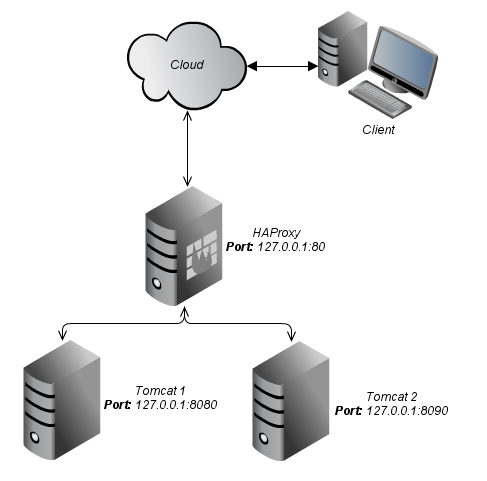
\includegraphics[width=0.9\textwidth]{figures/haproxy.png}
    \caption{The location of HAProxy in the system}
    \label{fig:haproxy}
\end{figure}

The following link reviews this solution in more detail:
\url{https://www.digitalocean.com/community/tutorials/an-introduction-to-haproxy-and-load-balancing-concepts}

\appendix

\section{Entry quiz sample questions}

\begin{enumerate}
    \item What is the difference between the public, private and hybrid cloud?
    \item What is IaaS, what are its attributes?
    \item What is OpenStack?
    \item What is the role of virtualization in cloud architecture?
    \item What are the main available settings at starting a VM using OpenStack?
    \item What do we call a Project in OpenStack, what functions are available on the online interface concerning a
          Project?
    \item How can we provide high availability for our service running in the cloud?
    \item What are the options for load-distributing algorithms at configuring HAProxy?
\end{enumerate}

\section{Lab exercises}

\subsection{Lab Introduction}

The task is configuring a Video service in OpenStack, with high availability. We perform the measurements in groups of
two. Start: Debian Jessie Live NFS 2015
The task is running a video server on a VM in the OpenStack cloud, in two settings: HTTP live streaming
and Video on Demand (RTSP). HTTP live streaming grants a continuous mediation, all clients connected to the server get
the same signal, while when using RTSP VoD every client sends a unique request to the server and can control the
replay.
Checking the performance with the VLC client. Then configuring the VMs started in multiple copies with
high availability and checking their performances.
OpenStack Dashboard interface: http://192.168.213.108/horizon
Login: labN/labN, where N=1..8
For the tasks there is a put-up image file available, with the VLC functioning as a client and video server with the
proper configuration files and the starting-stopping scripts already installed.

\subsection{Task 1.:Set-up}

Based to the OpenStack Dashboard syllabus
\begin{itemize}
\item create a virtual inner network (later connect the VM to this)
\item set up a security group, it's practical to open all TCP and UDP ports
\item create and assign an SSH key
\item create a virtual router, through which we connect the inner network to the global internet (ext-net)
\item set up a VM using the pre-built mereslab-vlc-v2 image
\begin{itemize}
\item m1.small flavor
\item It starts up slowly (about 2 minutes), the current status can be seen on the console, but first you need to type the following line into the /etc/hosts file:
         \emph{`controller1 192.168.213.108'}
\item Unfortunately, we can't log in through the console, only using SSH (from the local computer using an SSH key),
               you will also have to wait for logging in with SSH (about 1 minute)  
       username: ubuntu
\end{itemize}
\item Assign a Floating IP to the VM
\end{itemize}

\subsection{Task 2.:Starting and accessing the Video server}

The video server has to be started manually. Login to the VM using SSH, then:

\subsubsection{HTTP live streaming}
\textbf{Starter script:} \emph{`http\_streaming.sh'}

\noindent{}The HTTP stream is accessible through the following URL: http://{}\textless{}IP-address{}\textgreater{}:8888/live1 

\noindent{}\textbf{Task:} Open the video using our own computers. What IP-address is it accessible through? (You don't need to deal with the error messages concerning audio.)
Ask two other measuring groups to connect to our servers, and protocol the CPU load caused.

\noindent{}\textbf{Stopping HTTP streaming:} \emph{`sudo killall vlc'}

\subsubsection{RTSP VoD}
\textbf{Starter script:}  \emph{`rtsp\_streaming.sh'}

\noindent{}The RTSP stream is accessible through the following URL: rtsp://{}\textless{}IP-address{}\textgreater{}:5554/MyVideo

\noindent{}\textbf{Task:} Open the video using our own computers. (You don't need to deal with the error messages concerning audio.)
Ask two other measuring groups to connect to our servers, and protocol the CPU load caused.

\noindent{}\textbf{Stopping RTSP streaming:} sudo killall vlc

\subsection{Task 3.:Configuring high availability using HAProxy}

General description of setting up Load Balancing as a Service (LBaaS) in OpenStack:
\url{http://www.yet.org/2015/05/mos6-lbaas/}
From “Click on Load Balancers”, skipping the ``Add an HTTP Monitor" part, the ``Last but not least, add a VIP to your Pool" part is required, all the way until ``Web Instances", which is not.

\subsubsection{HTTP live streaming}

Create a Load Balance Pool for the HTTP live streaming servers, start at least two instances of VMs running the VLC server. In order to avoid manual operation of starting the video server, enter the following script -- that starts the VLC server –- at VM startup on the Post-Creation page:
\begin{lstlisting}[language=bash,breaklines]
#!/bin/bash
sudo -u ubuntu nohup /home/ubuntu/http_streaming.sh &
\end{lstlisting}

Organize the VM instances created into the formerly created Load Balance Pool. 

\noindent{}What do we experience when we are playing back on the local host? Through which IP-address is the Load Balance Pool accessible? Do the servers need a floating IP now? Why?

\noindent{}Ask two other measuring groups to connect to our HAProxy, and document the amount of CPU load on the servers caused by this.
Change the LB algorithm, test and compare the behaviors of these 3 variants!

\subsubsection{RTSP VoD}

Create a Load Balance Pool for the VoD RTSP streaming servers, start at least two instances of VMs running the VLC server, automate the startup of the VLC server like in the previous task, then organize the instances into the formerly created Load Balance Pool.

\noindent{}What do we experience when we are playing back on the local host? Can we see the video, the length of the video in the VLC player? What can cause this?

\noindent{}What can we see from the server loads? (Login to the server, using e.g. the "top" command.)

\noindent{}What types of traffic are there on the server? (Login to the server, using e.g. the "tcpdump" command.)

\end{document}